% #############################################################################
% This is Chapter 4
% !TEX root = ../main.tex
% #############################################################################
% Change the Name of the Chapter i the following line
\fancychapter{Planned Results}
%%%%%%%%%%%%%%%%%%%%%%%%%%%%%%%%%%%%%%%%%%%%%%%%%%%%%%%%%%%%%%%%%%%%%%%%
%                                                                      %
%     File: Thesis_Results.tex                                         %
%     Tex Master: Thesis.tex                                           %
%                                                                      %
%     Author: Francisco Azeredo                                        %
%     Last modified :  2 Jul 2015                                      %
%                                                                      %
%%%%%%%%%%%%%%%%%%%%%%%%%%%%%%%%%%%%%%%%%%%%%%%%%%%%%%%%%%%%%%%%%%%%%%%%
\label{chapter:Planned Results}
The planned results for this thesis, because it is a thesis given by a company is a final product. The product is a software program that aims to solve the problem of corporations that have large amounts of information stored in PDF documents and want that information to be readily available through an AI assistant. This program puts together a many different software techniques such as Vector Databases, \ac{LLM} to serve as AI assistants, \gls{RAG} systems that are already available but are not fully tested in this scenario or even known for it's comparative performance. 

This thesis aims to deliver a deployable software product designed to address the challenge faced by corporations managing extensive collections of information embedded within PDF documents. The proposed system provides seamless access to this information through an AI assistant interface, integrating state-of-the-art components including Vector Databases, Large Language Models (LLMs), and Retrieval-Augmented Generation (RAG) pipelines. The thesis further evaluates these technologies within the corporate document retrieval context, providing comparative performance insights and practical validation. 

\section{System Components}

\begin{itemize}
\item \textbf{Single Document AI Agent}: An LLM-powered agent capable of summarizing and interpreting individual documents in real time.
\item \textbf{RAG-based Document Retrieval Pipeline}: An end-to-end Retrieval-Augmented Generation (RAG) pipeline focused on scalable document storage and efficient, context-aware retrieval. The pipeline incorporates advanced integration techniques such as deduplication and conflict resolution (cf. DualRAG~\cite{Cheng2025}, CRP-RAG~\cite{Xu2024}), ensuring high-quality, non-redundant evidence is retrieved for downstream LLM processing.
\item \textbf{Document Metadata Generator}: An automated module that extracts and generates metadata to enhance document indexing and retrieval.
\item \textbf{AI Email Organizer}: An LLM-based agent that summarizes and categorizes incoming emails according to ongoing employee projects.
\end{itemize}

\section{Single Document AI Agent}
Rag pipeline explained: 
The methods used for this will be an llm, and a rag system. In here the single document must first be processed. 
Have add two levels of pre-processing, for a way to choose how much the document is processed, for the case where a fast processing is needed, level 2 or a slower but more comprehensive process which finds links between text to have a better context when text is retrieved. 
In both levels text chunking will be done the same way. Text will be split into sentences, and sentence are chunked to a certain amount of tokens.
In level 1, each chunk is embedded with an embedding model, vectorizing each chunk. Each chunk is then stored in a vector database.
In level 2, aside from level 1, each text chunk goes throuth a llm profiling process. A chunk is profiled to extract entities and keywords. That are then linked to that chunk. Then find if any other profiled chunk has the same entity and keyword. That will be a relashionship. And so the context of those two chunks is linked. This is saved in a graph database.
After pre-processing the document and having the vector embedding database and graph database of the document done.

\section{Single Document AI Agent}
The Single Document AI Agent combines LLMs with RAG pipelines to enable document-level semantic search and summarization. The system implements a configurable two-level pre-processing pipeline:

\begin{itemize}
\item \textbf{Level 1 (Fast Processing)}: The document is segmented into sentences and grouped into chunks of fixed token length. Each chunk is embedded using a vector embedding model and stored in a vector database for nearest neighboor search.
\item \textbf{Level 2 (Comprehensive Processing)}: In addition to Level 1, each chunk undergoes LLM-based profiling to extract entities and keywords. Chunks sharing entities or keywords are linked, forming relationships that are stored in a graph database to enhance contextual retrieval and semantic linkage.
\end{itemize}

This dual-level approach allows for trade-offs between processing speed and retrieval accuracy. After pre-processing, both the vector database and graph database representations of the document are available, enabling advanced, context-aware retrieval for downstream tasks.

\subsection{QA benchmark}
Testing with the embedding model all-MiniLM-L6-v2, and qwen2m models. For offline benchmarking. Here are the results, with all the available metrics. The heaviest but most important is bert based using the same all-MiniLM-L6-v2 embedding model to compare the gold answer and the model's answer. This test tests the capability of a knowledge graph used in mini and light, compared to the naive approach.

\begin{figure}[H]
    \centering
    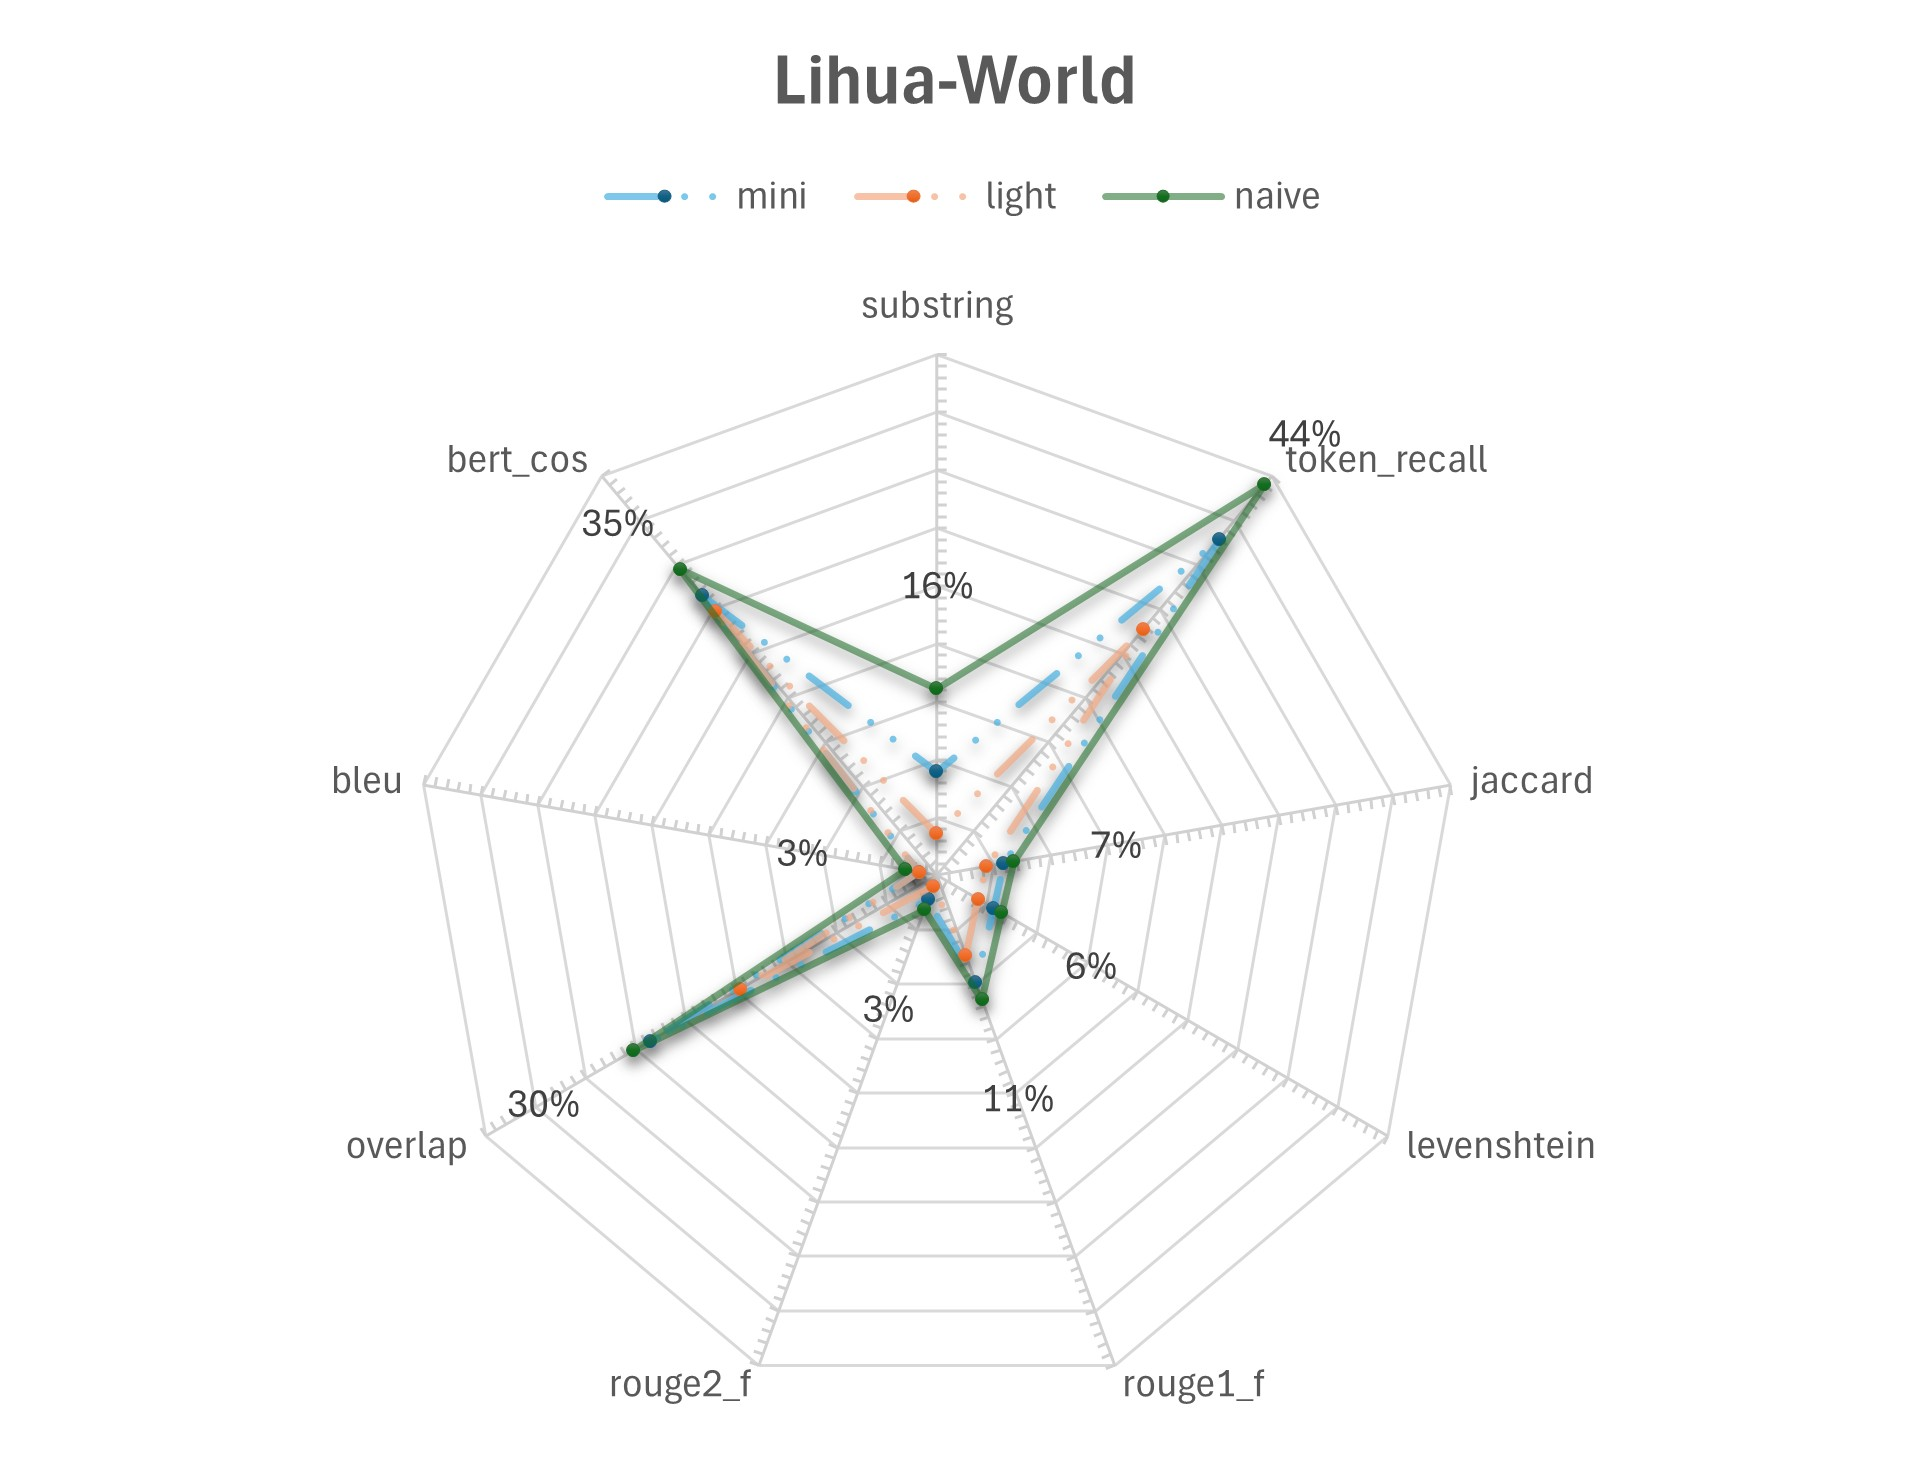
\includegraphics[width=1\linewidth]{Figures/Lihua-World.jpg}
    \caption{3 query types tested. With qwen2m as the llm and all-MiniLM-L6-v2 as embedding model}
    \label{fig:Lihua-World}
\end{figure}

\section{Final Product}
The final product \ref{fig:diagram_final} is an API designed for seamless interaction with documents and efficient retrieval of information through a \acrshort{llm}. In the user interface, authenticated users can securely log in and perform actions based on their permissions, such as uploading documents or querying the vector database through an AI assistant interface for allowed content, (e.g., "When did I meet Pedro?") and then receiving information of when Pedro was last met along with the last meeting logs. \\
In the backend, uploaded documents are processed to generate vector embeddings that capture their semantic meaning and are stored in a vector database optimized for fast similarity-based searches. Queries submitted by users are processed by the AI assistant, which employs vector search techniques to retrieve relevant information and delivers precise answers alongside supporting documents or excerpts. To ensure accuracy, the vector database is periodically updated offline, maintaining up-to-date content without disrupting the at inference operations. This architecture provides a secure, efficient, and user-friendly experience, enabling users to derive meaningful insights from their documents while maintaining a structured and scalable system.
\begin{figure}[H]
    \centering
    \includegraphics[width=1\linewidth]{Tese/images/Diagrama em branco.png}
    \caption{Simplified diagram of final product}
    \label{fig:diagram_final}
\end{figure}
\section{Comparative Analyzis}
Both in the part of process documents, and how documents will be stored different techniques will be used. The most relevant ones will be documented and compared throuth a few metrics.
\subsection{Evaluation metrics}
Here are the evaluation metrics that will be focused on document throuth the experiments of different techniques. And for also evaluating the program made in this thesis.
\begin{samepage}
\begin{itemize} 
\item \textbf{Offline Time:} The time required for a document to be processed and stored in the vector database. This includes embedding generation and insertion latency. 
\item \textbf{Inference Time:} The time between receiving a prompt and producing the output, measuring the real-time efficiency of the system during query processing. 
\item \textbf{Retrieval Precision:} The proportion of retrieved documents that are relevant to the query, evaluated using metrics such as Precision and Mean Reciprocal Rank (MRR). 
\item \textbf{Retrieval Recall:} The ability of the system to retrieve all relevant documents from the database for a given query, measured as Recall. \item \textbf{Answer Quality:} The accuracy and relevance of the generated output, assessed using human evaluation metrics. 
\item \textbf{Contextual Integration:} The model’s capability to effectively incorporate retrieved documents into the response, judged by the coherence and informativeness of the generated text. 
\item \textbf{Scalability:} The system’s ability to handle increasing database size and query load, measured by latency under stress tests with varying numbers of documents. 
\end{itemize}
\end{samepage}
\subsection{Context Analysis}
The program will also be tested for relevance in information retrieved by a query/prompt. Which i will create prompts that are supposed to fetch certain information from the documents that have been chosen carefully, with more detail in section \ref{sec:datasetcreation}
\subsection{External Benchmark}
\label{subsec:externalbenchmark}
An external benchmark will be used to evaluate the performance of the proposed RAG system. While there are many emerging benchmarks, a definitive choice has not yet been made. Among the options under consideration are the Loong Benchmark \cite{wang2024leavedocumentbehindbenchmarking}, which emphasizes long-context understanding through extended multi-document QA tasks; BEIR \cite{thakur2021beir}, a comprehensive suite of datasets designed to test retrieval and QA performance across various domains; and DocVQA \cite{mathew2021documentvisualquestionanswering}, which focuses on evaluating models' ability to extract and reason over document-based information. These benchmarks are particularly relevant to assessing the system's capacity for document retrieval, contextual integration, and accurate generation in a RAG framework.

\subsection{Benchmark Results}